\documentclass[twocolumn]{aastex631}

\usepackage{graphicx}
\usepackage{amsmath}
\usepackage{amssymb}
\usepackage{newtxtext,newtxmath}
\usepackage{hyperref}
\usepackage{gensymb}
\usepackage{enumitem}
\usepackage{booktabs}

\newcommand{\vdag}{(v)^\dagger}
\newcommand\aastex{AAS\TeX}
\newcommand\latex{La\TeX}

\newcommand{\Msun}{\ensuremath{M_{\odot}}}
\newcommand{\Gyr}{\ensuremath{\textrm{Gyr}}}
\newcommand{\Myr}{\ensuremath{\textrm{Myr}}}
\newcommand{\yr}{\ensuremath{\textrm{yr}}}
\newcommand{\kpc}{\ensuremath{\textrm{kpc}}}
\newcommand{\ckpc}{\ensuremath{\textrm{ckpc}}}
\newcommand{\pc}{\ensuremath{\textrm{pc}}}
\newcommand{\kms}{\ensuremath{\textrm{km}/\textrm{s}}}
\newcommand{\tocite}{\textcolor{blue}{cite}}
\newcommand{\FeH}{\ensuremath{[\textrm{Fe}/\textrm{H}]}}
\newcommand{\MgFe}{\ensuremath{[\textrm{Mg}/\textrm{Fe}]}}
\newcommand{\OFe}{\ensuremath{[\textrm{O}/\textrm{Fe}]}}
\newcommand{\alphaFe}{\ensuremath{[\alpha/\textrm{Fe}]}}
\newcommand{\tform}{\ensuremath{t_{\textrm{form}}}}
\newcommand{\dex}{\ensuremath{\textrm{dex}}}
\newcommand{\Msunyr}{\ensuremath{\Msun/\textrm{yr}}}
\newcommand{\Atmax}{\ensuremath{A_{2,\textrm{max}}}}

\newcommand{\rhalf}{\ensuremath{r_{\star,\textrm{half}}}}
\newcommand{\SFR}{\ensuremath{\textrm{SFR}}}

\newcommand{\red}[1]{\textcolor{red}{#1}}

\begin{document}

\title{Rising from the Ashes II: The Bar-driven Abundance Bimodality of the Milky Way}

\author{Angus Beane}
\affiliation{Center for Astrophysics $|$ Harvard \& Smithsonian, Cambridge, MA, USA}

\author{James W. Johnson}
\affiliation{Carnegie Science Observatories, Pasadena, CA, USA}

\author{Vadim Semenov}
\affiliation{Center for Astrophysics $|$ Harvard \& Smithsonian, Cambridge, MA, USA}

\author{Lars Hernquist}
\affiliation{Center for Astrophysics $|$ Harvard \& Smithsonian, Cambridge, MA, USA}

\author{Vedant Chandra}
\affiliation{Center for Astrophysics $|$ Harvard \& Smithsonian, Cambridge, MA, USA}

\author{Charlie Conroy}
\affiliation{Center for Astrophysics $|$ Harvard \& Smithsonian, Cambridge, MA, USA}

\begin{abstract}
    The Milky Way hosts at least two modes in its present day distribution of Fe and $\alpha$-elements. The exact cause of this bimodality is disputed, but one class of explanations involves the merger between the Milky Way and a relatively massive satellite (Gaia-Sausage-Enceladus) at $z\sim2$. However, reproducing this bimodality in simulations is not straightforward, with conflicting results on the prevalance, morphology, and mechanism behind multimodality. We present a case study of a galaxy in the Illustris TNG50 simulation which undergoes subsequent phases of starburst, brief quiescence, and then rejuvenation. This scenario results in a pronounced abundance bimodality after a post-processing adjustment of the \alphaFe{} of old stars designed to mimic a higher star formation efficiency in dense gas. The high- and low-$\alpha$ sequences are neatly separated in time by the brief quiescent period, which is not associated with a merger but by the formation of a bar followed by AGN activity. This galaxy indicates a novel scenario in which the $\alpha$-bimodality in the Milky Way is caused by the formation of the bar via AGN-induced quenching. In addition to a stellar age gap in the Milky Way, we predict that abundance bimodalities should be more common in barred as opposed to unbarred galaxies.
  \end{abstract}
    
  \keywords{Classical Novae (251) --- Ultraviolet astronomy(1736) --- History of astronomy(1868) --- Interdisciplinary astronomy(804)}

\section{Introduction}\label{sec:intro}
The stellar surface abundances of most elements retain the composition of their natal gas cloud. Therefore, the present-day distribution of their abundances encodes the chemical history of a galaxy's gas phase. Two classes of elements have received particular attention in the Milky Way due to their disparate formation channels: iron-peak (such as Fe) and $\alpha$-elements (produced through the $\alpha$-process, such as O and Mg). Enrichment of iron-peak elements is primarily through Type~Ia and Type~II supernovae (SNe), whereas enrichment of $\alpha$-elements is primarily only through Type~II SNe. In the Milky Way, there is a well-established bimodality with separate high- and low-$\alpha$ sequences as shown in the upper left panel of Figure~\ref{fig:fig1} \citep{1996ASPC...92..307G,1998A&A...338..161F,2004AN....325....3F,2006MNRAS.367.1329R,2011A&A...535L..11A,2012A&A...545A..32A,2014A&A...562A..71B,2014ApJ...796...38N,2020MNRAS.493.2952H}.

Broadly speaking, there are three approaches to explaining the bimodality. First, it is a result of internal secular processes that generate the bimodality through radial migration \citep{2009MNRAS.396..203S,2021MNRAS.507.5882S,2023MNRAS.523.3791C} or clump formation \citep{2019MNRAS.484.3476C,2020MNRAS.492.4716B,2021MNRAS.502..260B,2023ApJ...953..128G}. Second, the bimodality is generated through gas infall scenarios, either from specific gas accretion episodes from the intergalactic medium \citep{1997ApJ...477..765C,2009IAUS..254..191C,2017MNRAS.472.3637G,2019A&A...623A..60S}, or through a more self-consistent collapse sequence of the circumgalactic medium driven through feedback \citep{2021MNRAS.501.5176K}. Third and finally, the bimodality is generated through a merger process, either by enhancing the star formation rate (SFR) of the Galaxy \citep{2004ApJ...612..894B,2005ApJ...630..298B,2007ApJ...658...60B,2010MNRAS.402.1489R} or by supplying a relatively pristine gas supply that resets the metallicity of the Galaxy \citep{2020MNRAS.491.5435B,2024MNRAS.528L.122C}. Strong evidence that the Milky Way did undergo a merger with the Gaia-Sausage-Enceladus (GSE) satellite supports the merger-related scenarios \citep{2018MNRAS.478..611B,2018Natur.563...85H,2020ApJ...901...48N,2024ApJ...972..112C}.

In \citet{2024arXiv240707985B} (hereafter Paper~I), we proposed an alternate scenario for the formation of the bimodality, driven by a brief ($\sim300\,\Myr$) quiescent period in the Galaxy's history (an observational claim with a longer period of quiescence was made in \citet{2016A&A...589A..66H}). This period has two effects. First, the reduced SFR lowers the number of $\alpha$-producing Type~II SNe relative to Type~Ia\footnote{These SNe occur on different timescales (10s of Myr after star formation for Type~II, as compared to 100s of Myr to Gyrs for Type~Ia), so if the SFR drops, the number of Type~II SNe drops faster than Type~Ia.}, causing a sharp decline in the \alphaFe{} ratio in the star-forming gas. Second, the lower SFR results in fewer stars forming in the intermediate region between the high- and low-$\alpha$ sequences, reducing the occurrence of this transitional population in present-day observations. The combination of these two effects creates the valley between the high- and low-$\alpha$ sequences. This mechanism resembles two-phase infall models that incorporate a temporary halt in star formation \citep[][and references therein]{2024arXiv240511025S}, though the quiescent period in Paper~I is much shorter.

In Paper~I, we used idealized simulations of a galaxy merger that triggered the quiescent period. However, in that work we argued that it was the quiescent period, not the merger, which was necessary to produce a bimodality. In this work, we study a subhalo, or galaxy, from the Illustris TNG50 simulation demonstrating this. This galaxy exhibits the sequence of events presented in Paper~I after a post-processing step, motivated by recent work showing that the star formation efficiency (SFE) of dense gas at high-$z$ is too low in the TNG model \citep{2024arXiv240909121H}, which increases the \alphaFe{} of old star particles. The galaxy undergoes a brief quiescent period which neatly separates a high- and low-$\alpha$ sequence. However, instead of being preceded by a merger, the quenching is preceded by apparent bar-induced AGN activity. Therefore, this work serves as a verification that the scenario in Paper~I is possible in cosmological simulations and does not require a merger.

In Section~\ref{sec:methods}, we discuss our selection technique which led to discovering the galaxy, the observations we use for comparison, as well as a simple one zone chemical evolution model we use to justify our post-processing step. In Section~\ref{sec:results}, we present the main results which we discuss and interpret in Section~\ref{sec:disc}. We conclude in Section~\ref{sec:conc}.

\section{Methods}\label{sec:methods}
\subsection{IllustrisTNG Sample}\label{ssec:tng}
We use Illustris TNG50 \citep{2019MNRAS.490.3196P, 2019MNRAS.490.3234N, 2019ComAC...6....2N}, a cosmological simulation of a $\sim50\,\textrm{cMpc}$ box at high resolution ($m_{\textrm{baryon}}\sim8.5\times10^4\,\Msun$). It uses the gravito-magneto-hydrodynamics code \texttt{AREPO} \citep{2010MNRAS.401..791S, 2016MNRAS.455.1134P}, along with the TNG model \citep{2013MNRAS.436.3031V, 2017MNRAS.465.3291W, 2018MNRAS.473.4077P}. This model includes several subgrid processes, including a wind generation model, chemical enrichment from SNe and asymptotic giant branch stars, and thermal and kinetic feedback from AGN.

One piece of the TNG model of note for this work is the black hole (BH) accretion and feedback method \citep{2017MNRAS.465.3291W}. The BH accretion rate ($\dot{M}_{\textrm{BH}}$) is computed using the local structure of the gas phase with the Bondi-Hoyle-Lyttleton formula \citep{1939PCPS...35..405H,1944MNRAS.104..273B,1952MNRAS.112..195B}, with a maximum of the Eddington accretion rate ($\dot{M}_{\textrm{edd}}$). The model allows the BH to be either in a kinetic radio-mode or a thermal quasar-mode. If the Eddington ratio ($\dot{M}_{\textrm{BH}}/\dot{M}_{\textrm{edd}}$) exceeds a threshold ($M_{\textrm{BH}}$-dependent, but $\sim0.001$--$0.1$), the BH is in the quasar mode and injects a large amount of thermal energy into its surroundings.

Using the public catalog, we select a sample of subhalos at $z=1.5$ (snapshot 40) according to the following criteria: (1) the subhalo is central (i.e., the most massive subhalo within its halo), and (2) the subhalo's stellar mass is between $10^{10}$ and $10^{10.5}\,\Msun/\textrm{h}$. There were a total of 168 subhalos that met both criteria. The chosen mass range is broadly consistent with the expected mass of the Milky Way from abundance matching at this redshift \citep{2013ApJ...771L..35V}. We choose to make our selection of galaxies at $z=1.5$ instead of at lower redshift because we wish to capture the \textit{formation} of multimodal structure. Mergers at lower redshift contribute very little to the Milky Way's disk stars \citep[e.g.,][]{2016ARA&A..54..529B}, and would act as a contaminant in our sample.

We examine the abundance distribution in the \MgFe{}-\FeH{} plane for this sample of subhalos by visual inspection. Few subhalos display multimodal structure and, when present, is much weaker compared to that observed in the Milky Way. We then apply a post-processing step to the \MgFe{} of the stars, adding a value of $0.1\times\left(t_{1.5}-t_{\textrm{form}}\right)$ to each star particle, where $t_{1.5}$ is the age of the universe at $z=1.5$ ($\sim4.3\,\Gyr$), and $t_{\textrm{form}}$ is the formation time of the star particle. After this adjustment, which we justify in Section~\ref{ssec:sfe} based on TNG underpredicting the SFE of dense gas, we observe that the abundance structure becomes significantly more pronounced.

We show the abundance distributions (replicating Figure~\ref{fig:fig1}) of 16 random subhalos from our catalog, and the subhalo we selected, in Appendix~\ref{app:rand_fig1}. Of these subhalos, some structure is present, but none have a strong bimodality as seen in the Milky Way. After the $\alpha$-enhancement, a few have strongly bimodal features: 172175, 178140, 193025. It is worth noting that the post-processing is not in itself responsible for the emergence of bimodality, as it only does so for a fraction of the galaxies shown in Appendix~\ref{app:rand_fig1}. Furthermore, if a galaxy had \alphaFe{} slowly and continuously decrease with time, then our $\alpha$-enhancement would not give rise to a bimodality since it is also a continuous adjustment.

We select subhalo 172175 (the ID at snapshot 40) for its resemblance to the Milky Way. We then studied the main descendant of this subhalo at $z=0$ (subhalo 392276 at snapshot 99). A summary of its key properties is given in Table~\ref{tab:summ}.

% Please add the following required packages to your document preamble:
\begin{deluxetable}{lc}
  \tablecaption{Summary statistics of our subhalo of interest at $z=0$. $M_{200}$ and $R_{200}$ are relative to the mean density of the universe, the SFR is for all gas bound to the subhalo, and the BH refers to the central BH. \label{tab:summ}}
  \tablewidth{0pt}
  \tablehead{
    % \colhead{} & \colhead{}
  }
  \startdata
  \multicolumn{2}{c}{\textbf{dark matter}} \\ \hline
  $M_{200}$ & $4.97\times10^{12}\,\Msun$ \\
  $R_{200}$ & $532\,\kpc$ \\
  & \\
  \multicolumn{2}{c}{\textbf{baryons}} \\ \hline
  $\rhalf$ & $2\,\kpc$ \\
  $M_{\textrm{star}}(r<4\rhalf)$ & $7.6\times10^{12}\,\Msun$ \\
  $M_{\textrm{gas}}(r<4\rhalf)$ & $2.6\times10^{11}\,\Msun$ \\
  $\textrm{SFR}$ & $0.56\,\Msunyr$ \\
  $M_{\textrm{BH}}$ & $2.9\times10^{8}\,\Msun$ \\
  $\dot{M}_{\textrm{BH}}/\dot{M}_{\textrm{Edd}}$ & $4.5\times10^{-5}$ \\
  \enddata
\end{deluxetable}

\subsection{Observations}\label{ssec:obs}
We make use of two observational data sets. First, we use the stellar abundances from the ASPCAP pipeline of APOGEE DR17 \citep[][J.A.~Holtzman et al., in preparation]{2016AJ....151..144G,2017AJ....154...28B,2017AJ....154...94M,2022ApJS..259...35A}. We make the same selection cuts as in Section~2.4 of Paper I. These criteria select giants with high quality abundance measurements and angular momenta similar to the Sun's. This results in a sample of 54,777 stars. We use Fe to track total metallicity and Mg alone as an $\alpha$-element.

We then further considered a dataset of stellar ages from the APOKASC-3 catalog \citep{2024arXiv241000102P}. This catalog uses a combination of APOGEE spectroscopic parameters and \textit{Kepler} time series photometry to compute astroseismic ages. Using only stars with $25\%$ age uncertainties (taken as the maximum of the upper and lower uncertainty), we cross-match this catalog to our larger sample from ASPCAP which results in a sample of 2525 stars.

\subsection{One-Zone Chemical Evolution Model}\label{ssec:onezone_met}
One-zone galactic chemical evolution (GCE) models describe enrichment in an idealized gas reservoir in which newly synthesized metals mix instantaneously (see, e.g., the reviews by \citealt{Tinsley1980} and \citealt{Matteucci2021}). Our parameter choices in this paper are based on the models in \citet{2022arXiv220402989C}. While they were interested in bursts of star formation at the transition between the stellar halo and thick disk formation epochs, we focus on smooth evolutionary histories in this paper. We integrate these models numerically using the publicly available {\tt Versatile Integrator for Chemical Evolution} ({\tt VICE}; \citealt{2020MNRAS.498.1364J}).

The quantity of particular importance to our results is the depletion time $\tau_{\textrm{dep}}$, also known as the inverse of the star formation efficiency (SFE)\footnote{Note that the SFE we discuss here is averaged over a representative patch (e.g., kpc-size) and is not the dimensionless fraction of a giant molecular cloud that is converted into stars over its lifetime.} or the SFE timescale:
\begin{equation}
\tau_{\textrm{dep}} \equiv \frac{M_{\textrm{gas}}}{\SFR},
\end{equation}
where $M_{\textrm{gas}}$ is the mass of the gas reservoir. This timescale can be equivalently expressed as the ratio of the corresponding surface densities $\Sigma_{\textrm{gas}}$ and $\dot{\Sigma}_{\textrm{star}}$. $\tau_{\textrm{dep}}$ is the inverse of the SFE itself, describing the rate of star formation per unit gas mass. In principle, $\tau_{\textrm{dep}}$ should vary with $M_{\textrm{gas}}$ because the observed relation between $\dot{\Sigma}_{\textrm{star}}$ and $\Sigma_{\textrm{gas}}$ is non-linear; classically, $\dot{\Sigma}_{\textrm{star}} \propto \Sigma_{\textrm{gas}}^N$ where $N \approx 1.5$ (e.g. \citealt{Schmidt1959, Kennicutt1998}). For simplicity, we hold $\tau_{\textrm{dep}}$ constant in this paper, which corresponds to a linear relation. In Section~\ref{ssec:onezone} below, we present models using $\tau_{\textrm{dep}} = 0.5$, $1$, and $5\,\Gyr$.

Following \citet{2022arXiv220402989C}, our models assume that there is initially no gas present in the galaxy (i.e. $M_{\textrm{gas}} = 0$ at $t = 0$). Zero metallicity gas accretes at a constant rate of $\dot{M}_\text{in} = 5\,\Msunyr$. The efficiency with which feedback sweeps up interstellar material and ejects it to the circumgalactic medium in an outflow is described by the mass loading factor $\eta \equiv \dot{M}_\text{out} / \SFR$. We use $\eta = 2$ throughout this paper (i.e. for every solar mass of stars formed, $2\,\Msun$ of interstellar gas is lost to an outflow). These parameter choices lead to a SFH that initially rises from zero and approaches a constant value of $\sim1.9\,\Msunyr$. With these choices, the predicted abundance evolution is insensitive to the overall normalization of the accretion and star formation histories, since a larger accretion rate forms more stars and metals but simultaneously introduces more H into the interstellar medium.

We use the solar abundances of Fe and Mg from \citet{Magg2022} with an additional $0.04\,\dex$ to account for the effects of diffusion and gravitational settling (\citealt{Turcotte1998}; i.e. $\{Z_{\text{Fe},\odot}, Z_{\text{Mg},\odot}\} = \{13.7, 6.71\} \times 10^{-4}$). We adopt SN yields of Fe and Mg based on \citeauthor{Weinberg2023}'s \citeyearpar{Weinberg2023} recommendations for Type~II SNe:
\begin{itemize}

	\item $y_\text{Fe}^\text{II} = 4.73 \times 10^{-4}$

	\item $y_\text{Mg}^\text{II} = 6.52 \times 10^{-4}$

	\item $y_\text{Fe}^\text{Ia} = 12 \times 10^{-4}$

	\item $y_\text{Mg}^\text{Ia} = 0$,

\end{itemize}
where the subscripts and superscripts denote the element and SN type, respectively. We select this value of $y_\text{Fe}^\text{Ia}$ as it corresponds to $\sim30\%$ ($\sim70\%$) of Fe arising from Type~II (Ia) SNe at solar \FeH{}. These yields are population-averaged, meaning that they quantify the amount of metal production per unit mass of star formation under the given enrichment channel (e.g. a hypothetical $10^3\,\Msun$ stellar population would produce a total of $0.652\,\Msun$ of Mg through Type~II SNe). {\tt VICE} models Type~II SNe as exploding instantaneously following an episode of star formation. For Type~Ia SNe, we assume that metals are produced according to the empirically motivated $t^{-1.1}$ power-law based volumetric SN rates as a function of redshift and the cosmic SFH \citep[e.g.][]{Maoz2012}.

We use the yields recommended by \citet{Weinberg2023} because they are based on an empirical determination of the mean $^{56}$Ni yield from Type~II SNe by \citet{Rodriguez2021, Rodriguez2023} applied to multi-element abundance distributions in the Milky Way. Theoretically predicted SN yields \citep[e.g.][]{Seitenzahl2013, Sukhbold2016, Limongi2018, Gronow2021} are subject to substantial theoretical uncertainties. Empirical considerations regarding yields are often necessary for GCE models to make tenable predictions (see also discussion in \citealt{Palla2022}).

With the exception of our SN yields, we find through experimentation that the decline in \MgFe{} with time is most significantly sensitive to the value of $\tau_{\textrm{dep}}$. We therefore expect its connection to the decline in \MgFe{} on which this paper is focused to be robust. We refer to \citet{2020MNRAS.498.1364J} and \citet{2022arXiv220402989C} for further discussion of these GCE models.

\section{Results}\label{sec:results}
\subsection{Abundance Plane}\label{ssec:plane}

\begin{figure*}
  \centering
  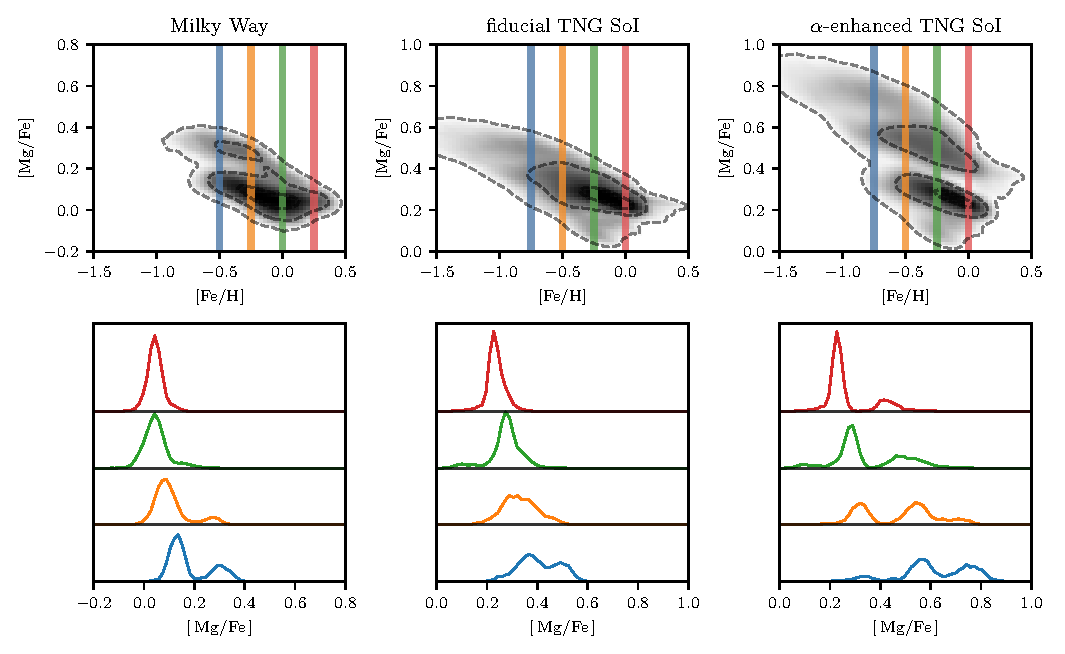
\includegraphics[width=\textwidth]{fig/392276.pdf}
  \caption{\textbf{When old stars are $\alpha$-enhanced, our subhalo of interest from TNG displays a prominent bimodality.} The upper left panel shows the distribution in the \MgFe{}-\FeH{} plane of the Milky Way, demonstrating a clear bimodality (data selection given in text). The lower left panel shows the 1D histograms of \MgFe{} at fixed \FeH{} values of $-0.5$, $-0.25$, $0$, and $0.25$ (blue, orange, green, and red, respectively). In the Milky Way, the bimodality is strongest at low metallicities while disappearing at high metallicities. The middle column shows the same plots but for our TNG subhalo of interest (392276) and with the fixed \FeH{} values $0.25\,\dex$ lower. Only faint structure is seen in the lowest bin (blue, $-0.75\,\dex$). The right column shows the same subhalo but after increasing the \MgFe{} value of star particles formed before $z=1.5$ linearly with formation time (with a slope of $0.1\dex/\Gyr$). A clear bimodality is shown in these panels which, unlike in the Milky Way, is present at all metallicities.}
  \label{fig:fig1}
\end{figure*}

The main result of our paper is given in Figure~\ref{fig:fig1}. Here, we compare the abundance plane in the Milky Way (left column) to that of our subhalo of interest (middle and right columns). The upper panels show the 2D distribution in the space of \MgFe{}-\FeH{}. We have applied the standard \texttt{scipy} implementation of a gaussian kernel density estimator to a Cartesian grid of points. For each panel, we normalize so that the integral of the distribution is unity. Colors are plotted in a log scale ranging from $0.08$ to $15\,\dex^{-2}$. Dashed contour lines are plotted at $0.1$, $1.5$, and $10\,\dex^{-2}$.

The colored vertical regions are indicated at $\FeH=-0.75$, $-0.5$, $-0.25$, and $0\,\dex$ in the Milky Way, and at bins $0.25\,\dex$ higher in the simulations. The lower panels show 1D histograms of \MgFe{} in bins centered on these values. The bins have width $0.1\,\dex$, which is reflected in the width of the colored, shaded regions in the upper panels. The rationale for the higher plotted \FeH{} in the simulations reflects the empirical location of the bimodalities. The Milky Way shows a clear bimodal population, with a high-$\alpha$ sequence most clearly distinct from the low-$\alpha$ sequence at low metallicity. The two sequences merge around solar metallicity.

Our galaxy, on the other hand, does not show a clearly bimodal structure in the fiducial simulation (middle column). There is some structure in the $\FeH=-0.75$ bin. The right panel of Figure~\ref{fig:fig1} shows the same distribution as in the middle panel, but with a modification to increase \MgFe{} values of older stars formed before $z=1.5$ (see Sections~\ref{ssec:tng} and \ref{ssec:onezone}). A multimodal structure emerges with three clear modes at $\MgFe\sim0.8$, $0.5$, and $0.2\,\dex$. The 1D histograms show that the modes are well-separated, and that the troughs between the modes nearly vanish.

\subsection{Alpha Time Dependence}\label{ssec:alpha_time}

\begin{figure*}
  \centering
  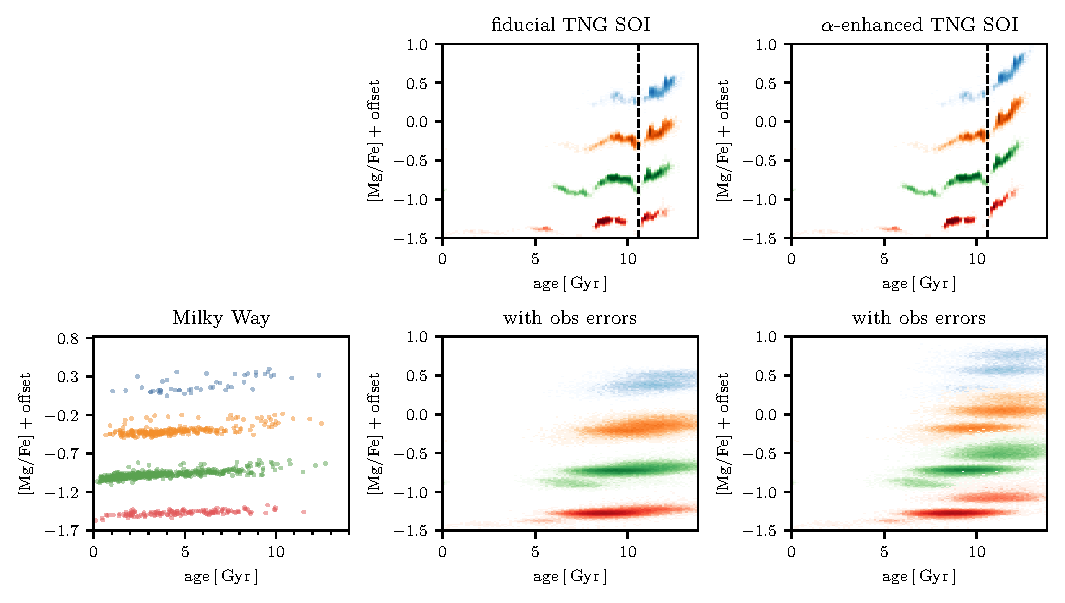
\includegraphics[width=\textwidth]{fig/392276_alpha.pdf}
  \caption{\textbf{Bimodality in the abundance plane is linked to distinct epochs in simulation.} The upper panels show \MgFe{} as a function of age for our subhalo in TNG. The colors indicate stellar populations at fixed values of \FeH{}, which are the same as in Figure~\ref{fig:fig1}. A gap in the relation occurs at an age of approximately $10.6\,\Gyr$, which we indicate with a vertical dashed line. The effect of the $\alpha$-enhancement is clear, as it separates the stars that form before and after this gap in ages (star particles which formed before $z=1.5$ are $\alpha$-enhanced, which occurs at an age of $\sim9.5\,\Gyr$). The lower panels show on the left the Milky Way and on the center and right the data from TNG but with $12.5\%$ age errors and $0.01\,\dex$ errors in \MgFe{}. When the simulations are given these errors, we see that the before and after star particles smear such that the two populations significantly overlap in ages. In the $\alpha$-enhanced galaxy, two populations emerge in each bin which overlapped in the fiducial distribution. This feature more closely resembles the Milky Way, which displays such populations where the bimodality is strongest -- $\FeH=-0.5$ (blue) and $-0.25$ (orange).}
  \label{fig:alpha}
\end{figure*}

The abundance distributions shown in Figure~\ref{fig:fig1} can be better understood by examining the evolution of \MgFe{} with time of the individual stars/star particles. In the upper panels of Figure~\ref{fig:alpha} we show the true distribution of \MgFe{} as a function of time for the fiducial galaxy in the middle and for the post-processed, $\alpha$-enhanced subhalo to the right. We use age instead of formation time in order to better facilitate comparisons to observations. These panels show 2D histograms, with a logarithmic colormap normalized to the maximum of the plot. To prevent overlap, the values of \MgFe{} are given offsets of $0$, $-0.5$, $-1$, and $-1.5$, in order of increasing \FeH{}.

In our galaxy, there is an age gap at $\sim10.6\,\Gyr$, which we mark with a vertical dashed line in the upper row. Star particles older than this line have a much clearer gradient in time with \MgFe{} than stars that form after. In the $\FeH=-0.25$ bin, star particles which form directly after this line have a slightly reduced \MgFe{} than stars which form a short time later.

In the lower row, the left panel shows data from the Milky Way, while the middle and right panels correspond to the fiducial and $\alpha$-enhanced galaxy, respectively. For the simulations, we introduce Gaussian errors of $12.5\%$ in age and $0.01\,dex$ in \MgFe{}. These error values align with the observational uncertainties from the APOKASC-3 and APOGEE datasets, which the Milky Way panel (lower left) is based on (see Appendix~\ref{app:obs_err} for detailed plots of observational errors). While the error in \MgFe{} is insignificant, the age error ($1.25\,\Gyr$ at $10\,\Gyr$) blurs the distribution, particularly around the dashed line that marks the transition between sequences. Despite this, the $\alpha$-enhanced galaxy still shows two distinct populations, although their ages now overlap more significantly.

The Milky Way distribution (lower left panel) exhibits some similarities to the $\alpha$-enhanced galaxy. Specifically, in the $\FeH=-0.5$ and $-0.25$ bins (blue and orange, respectively), there appear to be two populations that overlap in age but remain distinct in \MgFe{}. These are the bins where the bimodality is most pronounced (as seen in the upper left panel of Figure~\ref{fig:fig1}). In the Milky Way there also appears to be a population of $\alpha$-rich stars down to low ages (see discussion in Section~\ref{ssec:compare_obs}).

\subsection{Evolutionary History}\label{ssec:evol}
\begin{figure}
  \centering
  \includegraphics[width=\columnwidth]{fig/392276_SFH_AGN_M200.pdf}
  \caption{\textbf{The evolutionary history of our subhalo of interest.} The left column shows the SFH, BH accretion rate, and virial mass ($M_{200}$) over the entire time span, while the right column zooms in on the period from $t=2\,\Gyr$ to $t=5\,\Gyr$. The vertical dashed line in each panel marks the transition at $t\sim3.2\,\Gyr$, corresponding to the separation between the high- and low-$\alpha$ sequences (as shown in Figure~\ref{fig:alpha}). The upper panel shows the SFH, the middle panel shows the BH accretion rate as a fraction of the Eddington limit, and the lower panel shows the virial mass, representing the mass enclosed within a radius where the density is $200\times$ the mean cosmic density.}
  \label{fig:history}
\end{figure}

To understand the key events driving the behavior around the dashed line in Figure~\ref{fig:alpha}, we examine the evolution of several properties of our galaxy in Figure~\ref{fig:history}: its SFH, the BH accretion rate, and the growth of the virial mass. The vertical dashed line in each panel marks the transition at $t\sim3.2\,\Gyr$ from the high- to low-$\alpha$ sequences, as in Figure~\ref{fig:alpha}. The upper panel in the left column shows the the SFR (computed for all gas cells in the galaxy). There are two peaks at $t\sim2.5\,\Gyr$ and $t\sim4.5\,\Gyr$ with maximum values of $50\,\Msun/\textrm{yr}$ and $30\,\Msun/\textrm{yr}$, respectively. Around the high- to low-$\alpha$ transition, there is a dip in the SFR, which drops by an order of magnitude to about $3\,\Msun/\textrm{yr}$. The right panel zooms in on the period between $t=2\,\Gyr$ and $5\,\Gyr$, where we observe a sharp recovery in the SFR following the quiescent phase. In the span of a single snapshot (roughly $150\,\Myr$), the SFR increases from about $3\,\Msun/\textrm{yr}$ to $10\,\Msun/\textrm{yr}$.

The middle panels track the accretion rate of the central BH as a fraction of the Eddington rate. Early in our galaxy's history ($t<2\,\Gyr$), the BH experiences high accretion, which steadily declines until $t\sim5\,\Gyr$. Around $t\sim3.2\,\Gyr$, the BH accretion rate peaks again, reaching approximately $30\%$ of the Eddington limit, placing the BH in quasar mode and injecting significant thermal energy into the galaxy's center. The middle right panel shows the period between $t=2$ and $5\,\Gyr$. We can see that the decline in the galaxy's SFR is contemperaneous with this increase in the BH accretion rate.

The lower panel illustrates the growth of the galaxy's virial mass ($M_{200}$). Early on ($t<4\,\Gyr$), $M_{200}$ increases roughly linearly, reaching about $2 \times 10^{12}\,\Msun$. After this, the mass remains relatively stable until jumps occur around $t\sim10$ and $\sim12\,\Gyr$, indicative of mergers. These late-time mergers raise the virial mass to $5 \times 10^{12},\Msun$, well above the typical Milky Way estimate of $1$--$1.5\times 10^{12},\Msun$ \citep[e.g.][]{2016ARA&A..54..529B}. However, during the high- to low-$\alpha$ transition, the virial mass remains consistent with a Milky Way progenitor, making this galaxy a suitable analog. There are no mergers related to the earlier quiescent period around $t\sim3.2\,\Gyr$, as no major mass jumps are observed during this time. The lower right panel shows the lack of mergers in more detail during the period between $t=2$ and $5\,\Gyr$.

\subsection{Sequence of Events}\label{ssec:sequence_of_events}
\begin{figure*}
  \centering
  \includegraphics[width=\textwidth]{fig/alyssa.pdf}
  \caption{\textbf{Quiescence separating the high- and low-$\alpha$ sequences is preceded by AGN activity associated with bar formation.} Surface density projections of gas (top row) and star particles (middle row) in our galaxy across snapshots at different times during the high- to low-$\alpha$ transition. Below the projections is a plot showing the SFR, BH accretion rate (in units of $\dot{M}_{\textrm{BH}}/\dot{M}_{\textrm{edd}}$), and bar strength ($A_2/A_0$ for $R<2$ kpc). Time ranges from $\sim2.4\,\textrm{Gyr}$ to $\sim3.6\,\textrm{Gyr}$, corresponding to redshifts from $z\sim2.7$ to $z\sim1.8$. A sequence of events in which the bar strengthens, BH accretion increases, and SFR declines is seen, and is described more fully in the text.}
  \label{fig:seq}
\end{figure*}

In order to gain a more intuitive sense of the events around the high- to low-$\alpha$ transition, we show surface density projections alongside key summary statistics of our galaxy in Figure~\ref{fig:seq}. The upper panels show gas density, while the middle panels display stellar density. Time progresses from $\sim2.4$ to $\sim3.6\,\textrm{Gyr}$, corresponding to redshifts ranging from $z\sim2.7$ to $z\sim1.8$, and the high- to low-$\alpha$ transition is indicated with a vertical dashed line.

This figure shows the following sequence of events:
\begin{enumerate}
    \item Bar forms: A steady increase in the bar strength, as indicated by $A_2/A_0$ for star particles with $R<2\,\kpc$, from $\sim0.05$ to $0.4$ starting around $2.8\,\textrm{Gyr}$. This rise is accompanied by the appearance of elongated features in the gas and stars consistent with a bar.
    \item BH accretion increases: Following the increase in bar strength by about a snapshot ($\sim150\,\Myr$ here), the BH accretion rate ($\dot{M}_{\textrm{BH}}/\dot{M}_{\textrm{edd}}$) shows a significant spike, rising from a minimum of $\sim0.08$ at $t=2.84\,\Gyr$ to a maximum of $\sim0.29$ at $t=3.13\,\Gyr$ for one snapshot.
    \item SFR declines: The SFR declines starting from a maximum of $54.3\,\Msunyr$ at $t=2.84\,\Gyr$ down to $3.6\,\Msunyr$ at $t=3.28\,\Gyr$. In the next snapshot at $t=3.45\,\Gyr$ the SFR recovers to $12.2\,\Msunyr$. Figure~\ref{fig:history} shows that it reaches its second maximum of $30.9\,\Msunyr$ at $4.5\,\Gyr$.
\end{enumerate}

\subsection{One-Zone Model}\label{ssec:onezone}

\begin{figure}
  \centering
  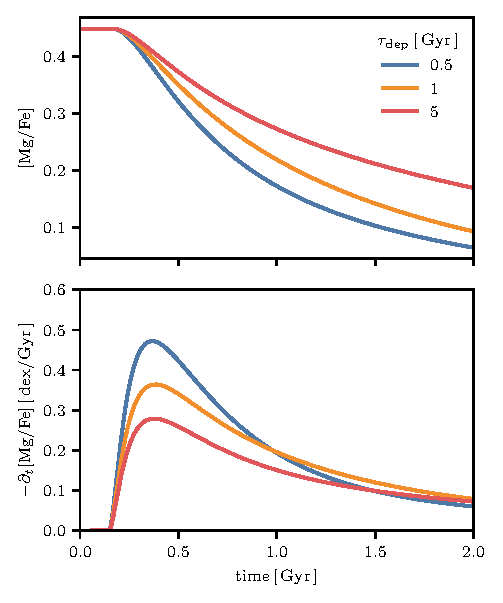
\includegraphics[width=\columnwidth]{fig/mgfe_vice.pdf}
  \caption{\textbf{A higher star formation efficiency leads to a steeper decline in \MgFe{}.} In both panels, the lines show the time evolution of \MgFe{} in a simple one-zone chemical evolution model, described in Section~\ref{ssec:onezone_met}. The evolution for different SFE values of $2$, $1$, and $0.2\,\textrm{Gyr}^{-1}$ are shown in blue, orange, and red, respectively.  The upper panel shows the evolution of \MgFe{} over $2\,\Gyr$, while the lower panel shows the negative of its time derivative. Increasing the SFE (decreasing $\tau_{\textrm{dep}}$) leads to a more rapid decline in \MgFe{}. At its steepest decline ($t\sim0.5\,\Gyr$), increasing the SFE by an order of magnitude results in a slope nearly twice as steep. At later times ($t > 1\,\Gyr$), models with higher SFE reach their steady-state \MgFe{} value more quickly.}
  \label{fig:vice}
\end{figure}

In Figure~\ref{fig:fig1}, we showed that a time-linear $\alpha$-enhancement of older stars (formed before $z=1.5$) leads to the emergence of a pronounced chemical bimodality. This $\alpha$-enhancement corresponds to a more rapid decline in \alphaFe{} over time at high redshifts. 
We demonstrate the physical motivation behind this $\alpha$-enhancement in Figure~\ref{fig:vice}.

The evolution of \MgFe{} in three one-zone GCE models with varying SFEs is shown in the upper panel of Figure~\ref{fig:vice} (models described in Section~\ref{ssec:onezone_met}). A higher SFE (lower $\tau_{\textrm{dep}}$) leads to a faster reduction in \MgFe{}. In the model with the highest SFE ($2\,\Gyr^{-1}$, $\tau_{\textrm{dep}}=0.5\,\Gyr$, blue), \MgFe{} drops from $\sim0.45$ to $0.08\,\dex$ over $2\,\Gyr$. In contrast, the model with the lowest SFE ($0.2\,\Gyr^{-1}$, $\tau_{\textrm{dep}}=5\,\Gyr$, red) only reaches $\sim0.2\,\dex$ within the same period.

The lower panel shows the negative time derivative of \MgFe{} (i.e., the rate of decline). The model with the highest SFE ($2\,\Gyr^{-1}$, blue) has a peak decline rate of $-0.5\,\dex/\Gyr$, while the model with the lowest SFE ($0.2\,\Gyr^{-1}$) peaks at $-0.25\,\dex/\Gyr$. After $1\,\Gyr$, the trend begins to reverse, and the lower-SFE models catch up, though at a much slower rate ($\sim-0.1\,\dex/\Gyr$) compared to their peak.

This analysis illustrates that a higher SFE at early times (high-$z$) leads to a faster decline in \MgFe{}. Recent work has suggested that the SFE in such dense regions in TNG may indeed be too low, as discussed in Section~\ref{ssec:sfe}. The post-processing $\alpha$-enhancement in Section~\ref{ssec:tng} is meant to mimic a SFE correction of high-$z$ dense gas.

\section{Discussion}\label{sec:disc}
In Figure~\ref{fig:fig1}, we compared the abundance plane between the Milky Way and our galaxy before and after our $\alpha$-enhancement post-processing procedure. It is clear that the TNG galaxy is unimodal before the $\alpha$-enhancement and multi-modal afterwards. Here, we briefly discuss two main points: (1) assuming the $\alpha$-enhancement is justified, what leads to the bimodality in the TNG galaxy?, and (2) what justifies the $\alpha$-enhancement? We then extend our comparison to data and argue the quiescent period is driven by a bar-induced AGN episode.

\subsection{Cause of Bimodality}\label{ssec:bim_cause}
We argue that the available evidence for the cause of the bimodality aligns with the scenario outlined in Paper~I. That study presented an idealized simulation resembling the merger between the Milky Way and GSE, where the orbital parameters were varied slightly across a grid of 27 simulations. The results showed that simulations featuring a brief quiescent period due to the merger produced a bimodal abundance distribution. In this scenario, gas expulsion by AGN activity was identified as the driving force behind the quenching.

Once the $\alpha$-enhancement post-processing has been done, the galaxy that we have studied in this work is consistent with the quiescent scenario proposed in Paper~I. The distribution of \MgFe{} with star particle age is a useful way to test this scenario, which we plot in the upper right panel of Figure~\ref{fig:alpha} in fixed bins of \FeH{} (each color is a different \FeH{} bin). The vertical dashed line in Figures~\ref{fig:alpha} and \ref{fig:history} marks the transition between the high- and low-$\alpha$ sequences. We place this transition at a lookback time of $10.6,\Gyr$, corresponding to a cosmic time of approximately $3.2,\Gyr$ or redshift $z\sim2.05$. \footnote{The transition between the high- and low-$\alpha$ sequences occurs approximately $1\,\Gyr$ before $z=1.5$, where the $\alpha$-enhancement begins. This, combined with the fact that not all of the subhalos in our sample display bimodalities (Appendix~\ref{app:rand_fig1}), shows that the $\alpha$-enhancement is not the direct cause of the bimodality.} Star particles formed before this transition show a steep decline in \MgFe{} over time, with a drop of approximately $0.3\,\dex$ in just $2\,\Gyr$. In contrast, the stars formed after the dashed line exhibit a much flatter trend, with no noticeable gradient in \MgFe{} for the next couple of Gyr.

At the transition, we can see a gap in the $\FeH=-0.5$, $-0.25$, and $0\,\dex$ bins (orange, green, and red, respectively). The gap has a width of about $300\,\Myr$ in the $-0.5$ and $-0.25\,\dex$ bins, while it is more extended at about $750\,\Myr$ in the $0\,\dex$ bin. The age gap in each \FeH{} bin of Figure~\ref{fig:alpha} is contemperaneous with a minimum in the global SFR. We can see in the upper panel of Figure~\ref{fig:history} that this dashed line lies almost exactly at the point of a local minimum in the SFH. This minimum, which is $\sim3\,\Msunyr$, is 10--15$\times$ smaller than the maxima before and after it.

During this period of suppressed SF, we argue that the lack of enrichment of Type~II relative to Type~Ia SNe leads to a lower rate of Mg production. The typical lifetime of a Type~II SN progenitor in this model is $\sim40\,\Myr$ \citep{2018MNRAS.473.4077P}, and so the hundreds of Myr of suppressed SF is short enough to restrict the production of $\alpha$-elements. Therefore, \MgFe{} rapidly declines. This, combined with a lack of SF in the first place, leads to a scarcity of star particles in the intermediate region between the high- and low-$\alpha$ sequences. A more in-depth explanation is given in Section~4.1 in Paper~I.

In the fiducial TNG distribution, shown in the upper middle panel of Figure~\ref{fig:alpha}, the same general behavior is present. However, because the \MgFe{} decline before the quiescent period is slower, star particles which formed before and after this period overlap in the \MgFe{} distribution shown in Figure~\ref{fig:fig1}.

Notably, both the fiducial and $\alpha$-enhanced galaxy show a slight rebound effect in \MgFe{}. The star particles which form directly after the dashed line when the SFR has just recovered have a slightly lower \MgFe{} than stars which form later on, by about $0.1$ to $0.2\,\dex$. This was also predicted in Figure~9 of Paper~I, where it was argued that during the period of suppressed star formation, the \alphaFe{} ratio of the star-forming gas drops sharply due to the reduced contribution of Type~II relative to Type~Ia SNe. Later, the \alphaFe{} of the gas will recover when the SFR also recovers, but there is a brief window when old, low-$\alpha$ stars can form. A similar behavior was seen in the one-zone models with bursty SFHs in \citet{2020MNRAS.498.1364J}.

\subsection{Steepening of $\alpha$ Decline}\label{ssec:sfe}
As described in Section~\ref{ssec:tng}, we applied a post-processing to the \MgFe{} of star particles in the TNG simulation. Specifically, for star particles formed before $z=1.5$, we added to their \MgFe{} a value of $0.1\times\left(t_{1.5}-t_{\textrm{form}}\right)$, where $t_{1.5}$ is the age of the universe at $z=1.5$ ($\sim4.3\,\Gyr$) and $t_{\textrm{form}}$ is the formation time. This post-processed subhalo is presented alongside the fiducial subhalo in the right and middle columns, respectively, of Figures~\ref{fig:fig1} and \ref{fig:alpha}.

The \MgFe{} value of star forming gas is the result of a complicated mixture of many different aspects of the TNG model, to name a few: stellar and AGN feedback which alter gas inflows and outflows, secular, dynamical evolution, SF prescription, magnetic fields, (lack of) cosmic rays, diffusivity of hydrodynamics solver, and, of course, enrichment models. Isolating the cause of the ``incorrect''\footnote{Our case study of a single subhalo, selected in a non-reproducible manner, is hardly cause to firmly assert that the fiducial evolution in TNG50 is incorrect.} \MgFe{} vs. time evolution at high-$z$ is not straightforward nor, in our opinion, even possible. However, we do offer one reasonable explanation: the SFE at high densities, more present at high-$z$, is too low.

We demonstrate the impact of the SFE on the \alphaFe{} ratio using a simple one-zone chemical evolution model with the publicly available code \texttt{VICE}. The details of our setup is given in Section~\ref{ssec:onezone_met}. We vary the SFE of the model ($\textrm{SFR}/M_{\textrm{gas}}$), and examine the impact on \MgFe{} as a function of time. We find that a higher SFE does lead to a more rapid reduction in \MgFe{}. The rate of decrease in \MgFe{}, at its maximum, varies between $\sim-0.25$, $-0.35$, and $-0.5\,\dex/\Gyr$ in the $\textrm{SFE}=0.2$, $1$, and $2\,\Gyr^{-1}$ models, respectively. For our post-processing, we assumed an additional decrease rate of $0.1\,\dex/\Gyr$. Such a difference is well within the range of \MgFe{} slopes seen in our different $\tau_{\textrm{dep}}$ models, implying a factor of only $\sim2$ to $5$ in the SFE is needed to reach our post-processing slope.

\citet{2024arXiv240909121H} demonstrated that the pressure regulated feedback model of \citet{2022ApJ...936..137O} predicts higher SFRs of patches of gaseous disks in TNG50 than the fiducial model by up to an order of magnitude. This is well within our needed factor of $\sim2$ to $5$ in the SFE (see Figure~\ref{fig:vice}). Therefore, \MgFe{} should decline more rapidly with a different feedback model (or future iteration of the TNG model) that leads to a higher SFE at high densities.

An intuitive understanding of the impact the decline in \alphaFe{} vs. time has is that, when \alphaFe{} declines rapidly, it is a better estimator of age. When \alphaFe{} is a better estimator of age, events which are separated temporally become better separated in the abundance plane.

\subsection{Direct Comparison to Observations}\label{ssec:compare_obs}
The lower left panel of Figure~\ref{fig:alpha} shows the \MgFe{} vs. age of stars in bins of \FeH{} which pass our solar neighborhood selection and are present in the APOKASC-3 catalog. In the bins where the bimodality is strongest (blue and orange, $\FeH=-0.5$ and $-0.25$, respectively), we see that there is a sort of two tiered distribution with significant overlap in age. In the galaxy with age and abundance errors shown in the lower right panel, a similar distribution can be seen in all \FeH{} bins. An examination of the true distribution in the galaxy (upper right panel), we see that the two distributions are in fact very cleanly separated in age.

There is also a population of young, $\alpha$-rich stars in the APOKASC-3 data. These may or may not reflect the typical or average ISM chemistry. Arguments have been made that they are old stars with misclassified astroseismic ages due to binary mass transfer \citep[and references therein]{2023A&A...671A..21J}. However, some appear to be genuinely young \citep[and references therein]{2024arXiv241002962L}, with a range of explanations given \citep[e.g.][]{2015A&A...576L..12C,2021MNRAS.508.4484J,2023arXiv231105815S}. Disentangling these effects is far from clear and beyond the scope of this work. At least some of the young, $\alpha$-rich stars in Figure~\ref{fig:alpha} do not reflect the ISM chemistry at their inferred astroseismic age, and so would not be included in the TNG model. With this caveat, the two appear to be consistent.

\subsection{Cause of Quiescence}\label{ssec:cause_qui}
In Paper~I, AGN activity from a merger was the suspected cause for the quiescent period. In our galaxy here, there is indeed a brief burst in AGN accretion at the time of the merger (middle panel of Figure~\ref{fig:history}). Based on this burst, it is also reasonable to suspect that AGN activity is also responsible for the quiescent period in our galaxy. However, we argue that the cause of the localized spike in the BH accretion rate is not due to a merger but instead due to the formation/strengthening of a bar.

In Figure~\ref{fig:seq}, we combine a visual inspection of the gas (upper row) and stellar (middle row) surface densities with the evolution of three key quantites (lower plot): SFR, BH accretion rate, and bar strength in blue, orange, and red, respectively. These are shown for nine snapshots, from snapshot 27 to 35, corresponding to redshift $2.73$ to $1.82$ or cosmic time from $2.38\,\Gyr$ to $3.59\,\Gyr$. A vertical dashed line is included in the lower panel separating the formation of the low- and high-$\alpha$ sequence at an age of $10.6\,\Gyr$ (cosmic time $\sim3.2\,\Gyr$), as in Figures~\ref{fig:alpha} and \ref{fig:history}.

As described in Section~\ref{ssec:sequence_of_events}, the bar strengthens and then the BH accretion rate spikes, all while the SFR of the galaxy declines. This is suggestive of the following causal sequence:
\begin{enumerate}
  \item a bar forms through an internal instability, which
  \item drives a large amount of gas to the center of the galaxy, which
  \item triggers a high BH accretion rate and quasar-mode thermal feedback, which
  \item clears gas out of the galaxy leading to quiescence.
\end{enumerate}
This quiescent period then leads to the bimodality, as discussed in Section~\ref{ssec:bim_cause}. It is not possible to prove the causality of this sequence of events because of the sparse snapshot spacing in TNG50, and so this is left to future work.

However, there is a significant body of theoretical and observational work in support of this picture. Bars and other non-axisymmetric features have long been argued to funnel gas into the centers of galaxies on theoretical grounds \citep{1989Natur.338...45S,2010MNRAS.407.1529H}. It was recently shown by \citet{2024arXiv240906783F} that bars can induce quiescence by accelerating the growth of a SMBH, but they found there can be many Gyr between bar formation and quenching. In observations, barred galaxies preferentially host AGN in star-forming galaxies \citep{2012ApJS..198....4O,2022A&A...661A.105S}.\footnote{\citet{2022A&A...668L...3L} studied a galaxy from TNG100 in which a merger induced AGN activity that ejected gas from its center. A bar then formed out of the gas-poor disk.} Furthermore, at high-$z$, the AGN mechanism is thought to be responsible for quenching \citep[e.g.][and references therein]{2023arXiv230806317D,2024arXiv240417945P,2024arXiv240518685M,2024Natur.630...54B}.

Since barred galaxies preferentially host AGN, we therefore predict that barred galaxies would preferentially host $\alpha$-bimodalities. The GECKOS survey, which aims to constrain the $\alpha$-bimodality of edge-on galaxies using integral field spectroscopy at different altitudes, could test this \citep{2024IAUS..377...27V}. On the other hand, the strength of a bar is not associated with the strength of the host AGN \citep[e.g.]{2022A&A...661A.105S}. So, it is not clear that bimodalities would be associated with bar strength.

A complicating factor for this picture comes from the high SFR associated with the galaxy. The depletion time ($M_{\textrm{gas}}/\textrm{SFR}$) at the $t=2.84\,\Gyr$ snapshot is $204\,\Myr$, shorter than the time it takes for the SFR to reach its minimum. This implies the possibility of starvation as a quenching mechanism. However, the average depletion time in the preceding 5 snapshots (which are each $\sim150\,\Myr$ apart) is $220\,\Myr$, so clearly the galaxy is accreting high amounts of gas from its environment. A definitive account, difficult with the current simulation outputs because of its sparse snapshot spacing, requires further work.

\section{Conclusions}\label{sec:conc}
In this work, we examined a subhalo of interest in Illustris TNG50. This galaxy is at a Milky Way-progenitor mass at $z=1.5$. After applying a post-processing step that increased the \MgFe{} of star particles formed before $z=1.5$, this subhalo hosts a strong bimodality in the plane of \MgFe{} and \FeH{}, shown in Figure~\ref{fig:fig1}. This post-processing is justified by arguing that the SFE of dense gas is too low in TNG \citep[][see discussion in our Section~\ref{ssec:sfe}]{2024arXiv240909121H}.

This bimodality can be traced to an event that occurred at an age of $10.6\,\Gyr$, or cosmic time of $\sim3.2\,\Gyr$ ($z\sim2$). Shown as a vertical dashed line in Figure~\ref{fig:alpha}, star particles that form before this time are at high-\MgFe{}, while star particles that form after are at low-\MgFe{}. This time is associated with a global reduction in the SFR (Figure~\ref{fig:history}), which appears to be related to AGN activity induced by the formation of a bar (Figure~\ref{fig:seq}).

We argue that the reduction in the SFR has two effects which lead to the $\alpha$-bimodality. First, a lower production of Mg relative to Fe is the natural result of a lack of Type~II relative to Type~Ia SNe. The latter remain high due to their longer timescales, expediting a drop in \MgFe{}. Second, the lack of SF means that stars at \MgFe{} intermediate between the high- and low-$\alpha$ sequences never form. This argument is the same as presented in Paper~I and is consistent with the one-zone chemical evolution models of \citet{2020MNRAS.498.1364J}. When observational errors are added to the subhalo's abundance vs. age distribution, we show that it is broadly consistent with the distribution observed in the Milky Way (Figure~\ref{fig:alpha} and Section~\ref{ssec:compare_obs}).

This work adds further support to a scenario in which a quiescent period in the Milky Way's past is a plausible explanation for the Milky Way's abundance bimodality. We argued in Paper~I that the GSE merger could trigger this period. In this work we have argued that the formation of the Milky Way's bar could be responsible. Regardless of this scenario's relevance to the Milky Way, we also predict that the presence of a bar in external galaxies is correlated with the presence of an $\alpha$-bimodality.

\begin{acknowledgements}
This work has made use of data from the European Space Agency (ESA) mission {\it Gaia} (\url{https://www.cosmos.esa.int/gaia}), processed by the {\it Gaia} Data Processing and Analysis Consortium (DPAC, \url{https://www.cosmos.esa.int/web/gaia/dpac/consortium}). Funding for the DPAC has been provided by national institutions, in particular the institutions participating in the {\it Gaia} Multilateral Agreement.
\end{acknowledgements}

\bibliography{ref}{}
\bibliographystyle{aasjournal}

\appendix

\section{Observational Errors}\label{app:obs_err}
In Figure~\ref{fig:alpha}, we assumed observational errors of $12.5\%$ in age and $0.01\,\dex$ in \MgFe{}. In Figure~\ref{fig:obs_err}, we plot the quoted observational errors of the APOKASC-3 (left) and ASPCAP (right) datasets, showing both \FeH{} and \MgFe{} (blue and orange, respectively). We show our $12.5\%$ age error and $0.01\,\dex$ abundance error assumptions as black lines. For the age error, we used the maximum of the upper and lower estimates from \citet{2018ApJS..239...32P}. As a dashed line we show our $25\%$ age error cut for stars plotted in Figure~\ref{fig:obs_err}. Our assumed errors are generally consistent with the observed. Our error in \MgFe{} is a bit smaller than in ASPCAP, but the age estimates are by far the more constraining of the two.

\begin{figure*}
  \centering
  \includegraphics[width=\columnwidth]{fig/obs_error.pdf}
  \caption{The observational errors of the APOKASC-3 (left) and ASPCAP dataset (right). We show, on the left, a line indicating a $12.5\%$ error in observed age and on the right a vertical line indicating a $0.01\,\dex$ error. On the left, a dashed line indicates the $25\%$ error cut used for inclusion in Figure~\ref{fig:alpha}.}
  \label{fig:obs_err}
\end{figure*}

\section{Random Selection of Subhalos}\label{app:rand_fig1}
In Figures~\ref{fig:app0} to \ref{fig:app16}, we show a version of Figure~\ref{fig:fig1} but for a random selection of subhalos from our broader sample of 168 Milky Way-progenitors at $z=1.5$ in TNG50. It is from this sample that we selected our galaxy of interest. We first show this galaxy at $z=1.5$ in Figure~\ref{fig:app0}, and then show our random sample of 16.

\begin{figure*}
  \centering
  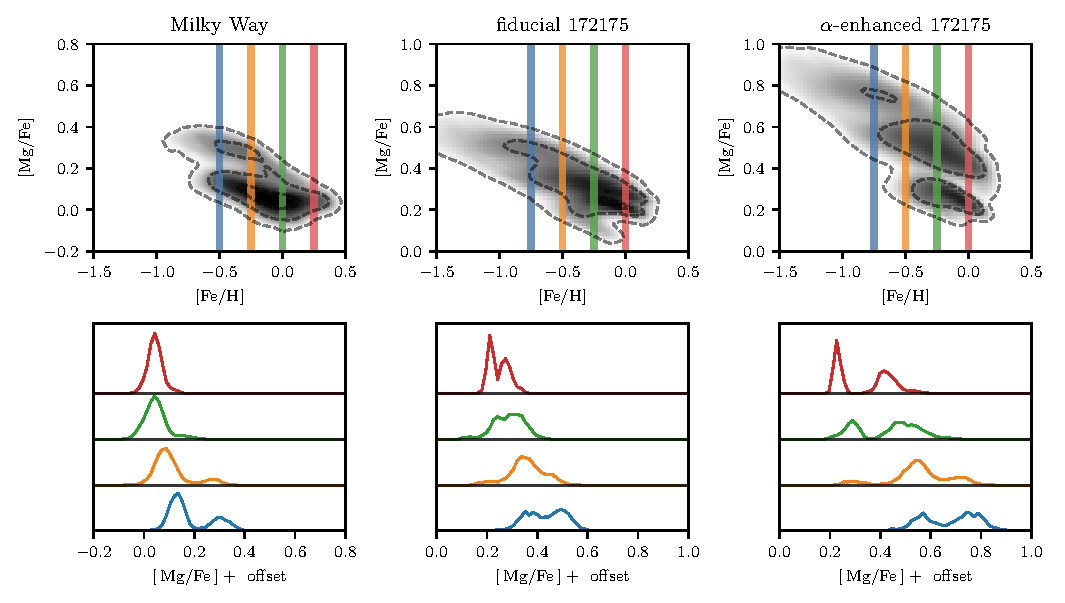
\includegraphics[width=\textwidth]{fig/app_172175.pdf}
  \caption{The same as Figure~\ref{fig:fig1}, but for our galaxy of interest at $z=1.5$.}
  \label{fig:app0}
\end{figure*}

\begin{figure*}
  \centering
  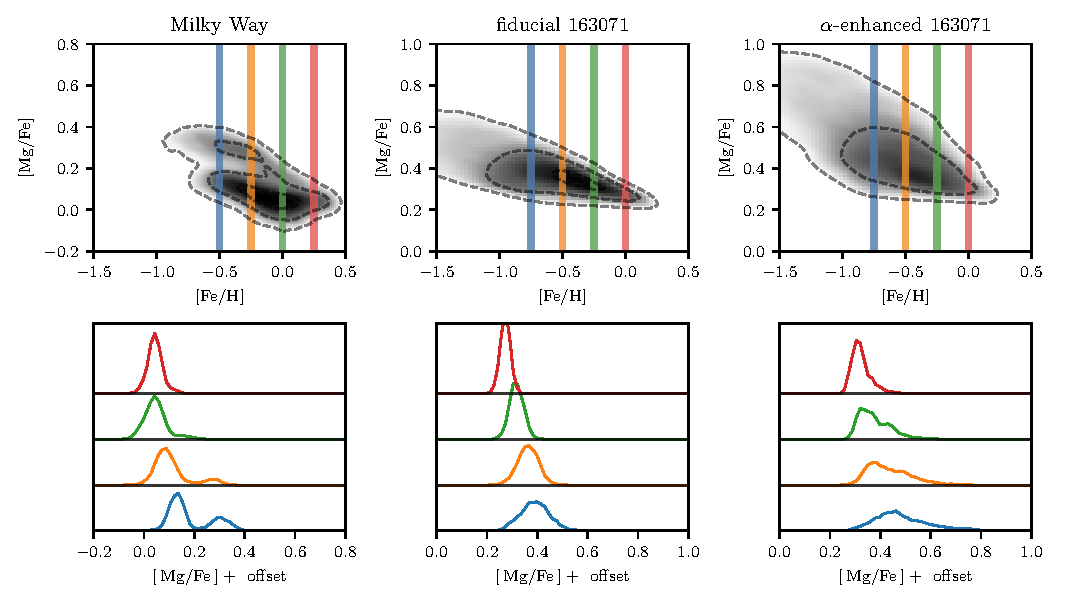
\includegraphics[width=\textwidth]{fig/app_163071.pdf}
  \caption{The same as Figure~\ref{fig:fig1}, but for a random subhalo from our catalog at $z=1.5$.}
  \label{fig:app1}
\end{figure*}

\begin{figure*}
  \centering
  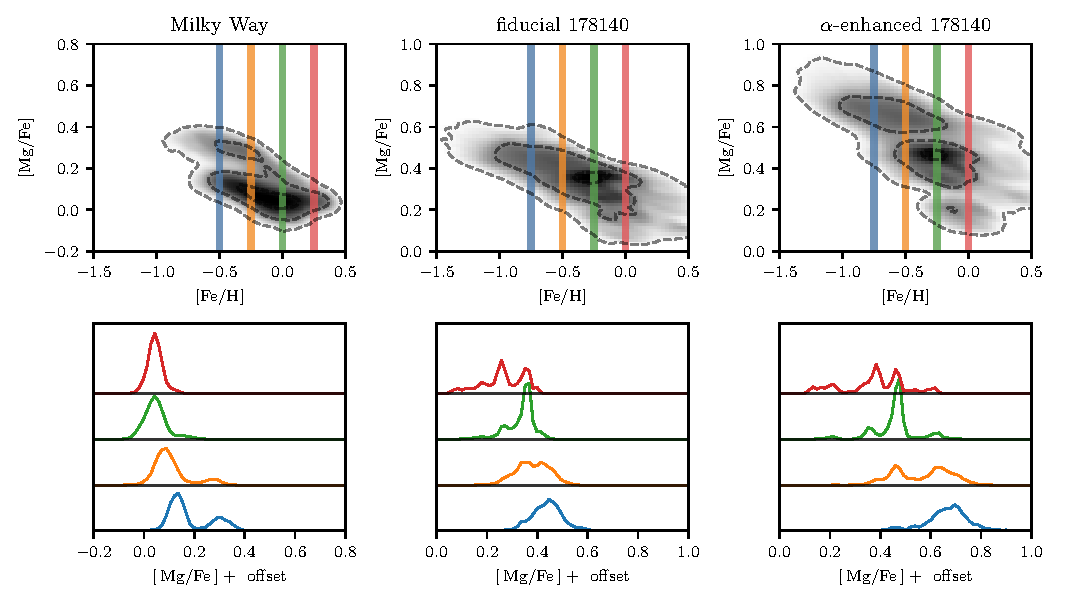
\includegraphics[width=\textwidth]{fig/app_178140.pdf}
  \caption{The same as Figure~\ref{fig:fig1}, but for a random subhalo from our catalog at $z=1.5$.}
  \label{fig:app2}
\end{figure*}

\begin{figure*}
  \centering
  \includegraphics[width=\textwidth]{fig/app_179009.pdf}
  \caption{The same as Figure~\ref{fig:fig1}, but for a random subhalo from our catalog at $z=1.5$.}
  \label{fig:app3}
\end{figure*}

\begin{figure*}
  \centering
  \includegraphics[width=\textwidth]{fig/app_193025.pdf}
  \caption{The same as Figure~\ref{fig:fig1}, but for a random subhalo from our catalog at $z=1.5$.}
  \label{fig:app4}
\end{figure*}

\begin{figure*}
  \centering
  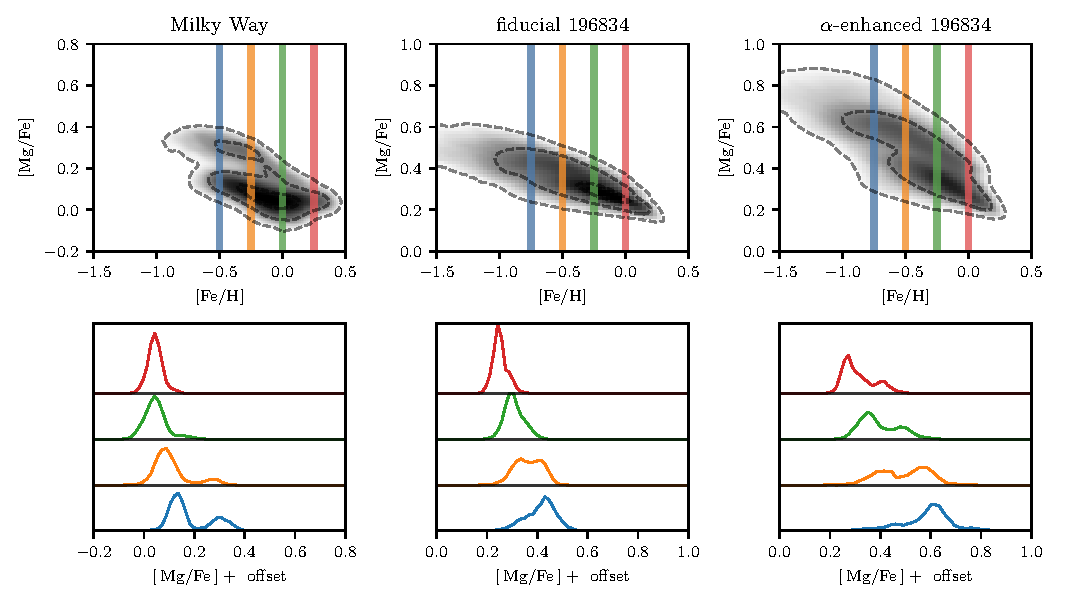
\includegraphics[width=\textwidth]{fig/app_196834.pdf}
  \caption{The same as Figure~\ref{fig:fig1}, but for a random subhalo from our catalog at $z=1.5$.}
  \label{fig:app5}
\end{figure*}

\begin{figure*}
  \centering
  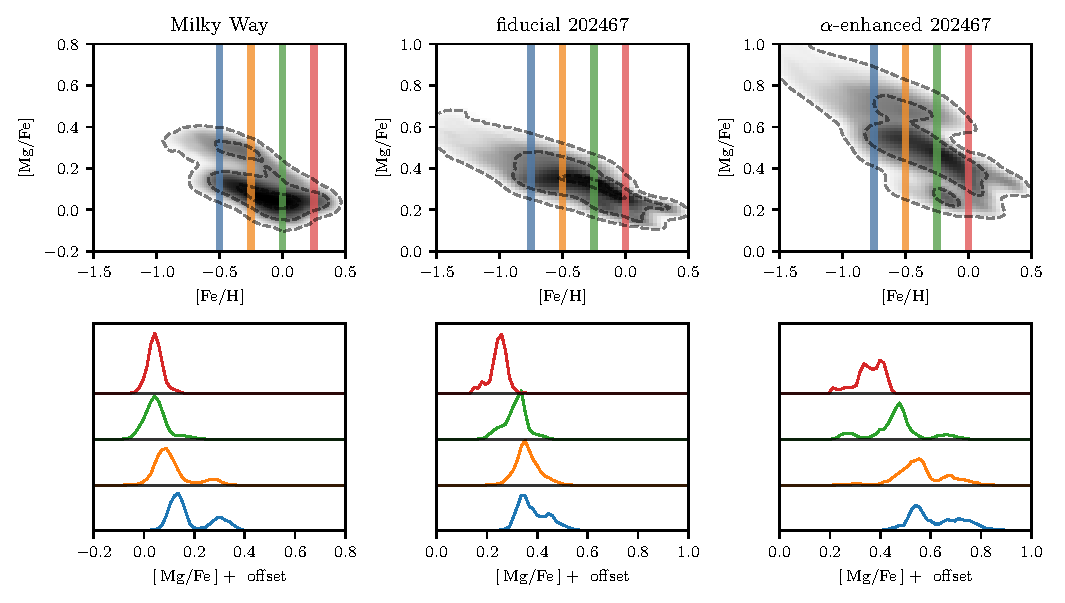
\includegraphics[width=\textwidth]{fig/app_202467.pdf}
  \caption{The same as Figure~\ref{fig:fig1}, but for a random subhalo from our catalog at $z=1.5$.}
  \label{fig:app6}
\end{figure*}

\begin{figure*}
  \centering
  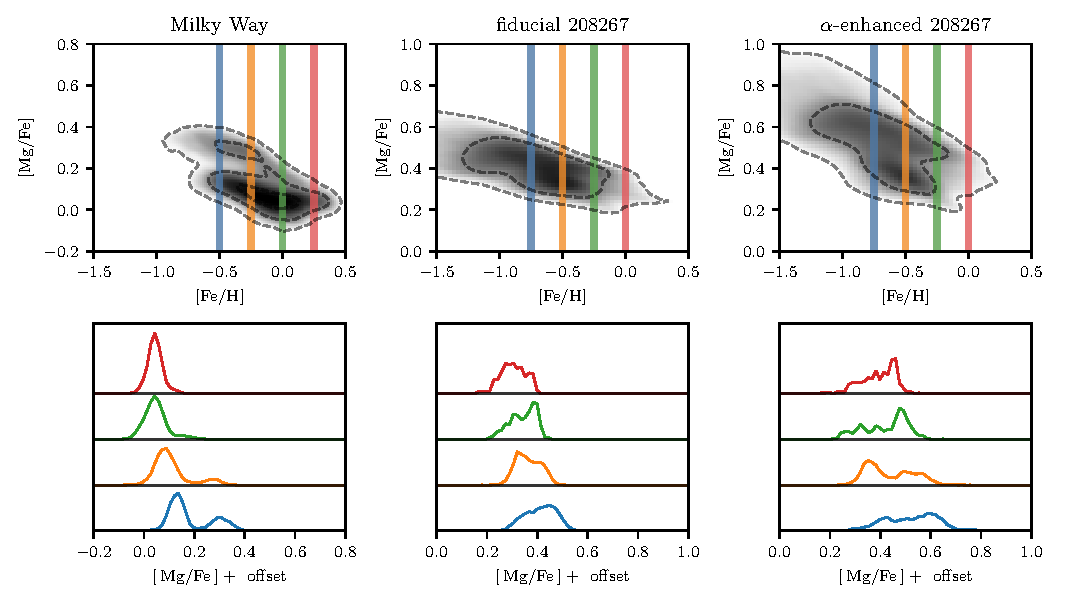
\includegraphics[width=\textwidth]{fig/app_208267.pdf}
  \caption{The same as Figure~\ref{fig:fig1}, but for a random subhalo from our catalog at $z=1.5$.}
  \label{fig:app7}
\end{figure*}

\begin{figure*}
  \centering
  \includegraphics[width=\textwidth]{fig/app_222555.pdf}
  \caption{The same as Figure~\ref{fig:fig1}, but for a random subhalo from our catalog at $z=1.5$.}
  \label{fig:app8}
\end{figure*}

\begin{figure*}
  \centering
  \includegraphics[width=\textwidth]{fig/app_235345.pdf}
  \caption{The same as Figure~\ref{fig:fig1}, but for a random subhalo from our catalog at $z=1.5$.}
  \label{fig:app9}
\end{figure*}

\begin{figure*}
  \centering
  \includegraphics[width=\textwidth]{fig/app_245661.pdf}
  \caption{The same as Figure~\ref{fig:fig1}, but for a random subhalo from our catalog at $z=1.5$.}
  \label{fig:app10}
\end{figure*}

\begin{figure*}
  \centering
  \includegraphics[width=\textwidth]{fig/app_254663.pdf}
  \caption{The same as Figure~\ref{fig:fig1}, but for a random subhalo from our catalog at $z=1.5$.}
  \label{fig:app11}
\end{figure*}

\begin{figure*}
  \centering
  \includegraphics[width=\textwidth]{fig/app_260347.pdf}
  \caption{The same as Figure~\ref{fig:fig1}, but for a random subhalo from our catalog at $z=1.5$.}
  \label{fig:app12}
\end{figure*}

\begin{figure*}
  \centering
  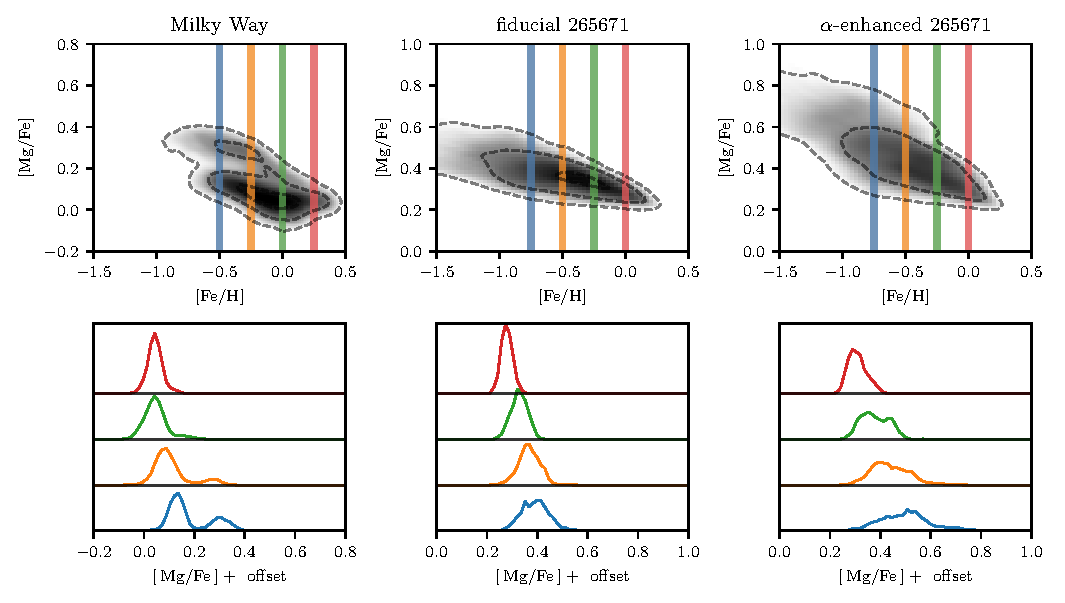
\includegraphics[width=\textwidth]{fig/app_265671.pdf}
  \caption{The same as Figure~\ref{fig:fig1}, but for a random subhalo from our catalog at $z=1.5$.}
  \label{fig:app13}
\end{figure*}

\begin{figure*}
  \centering
  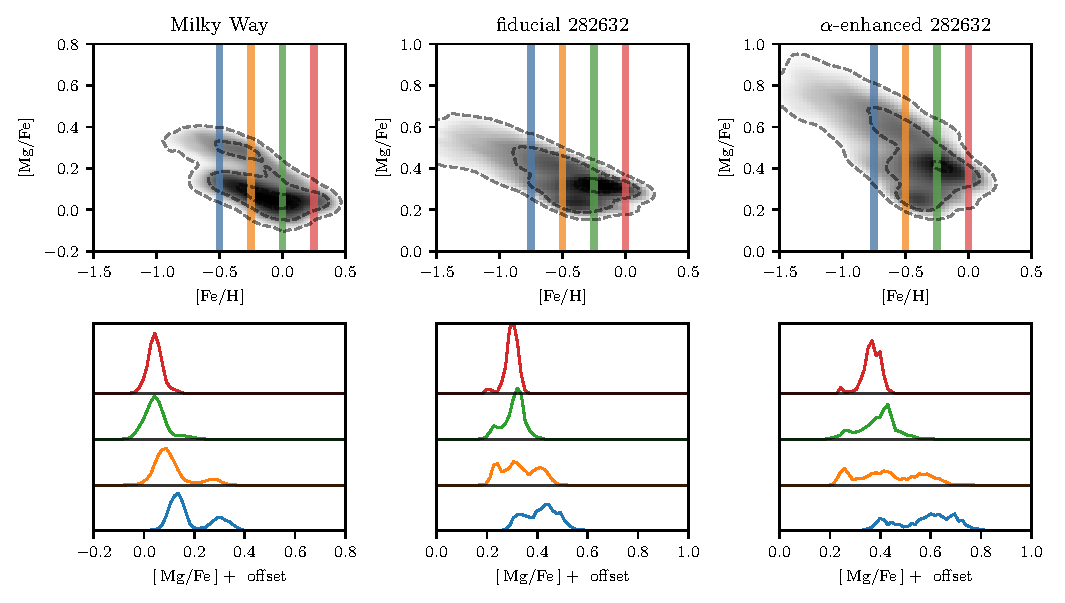
\includegraphics[width=\textwidth]{fig/app_282632.pdf}
  \caption{The same as Figure~\ref{fig:fig1}, but for a random subhalo from our catalog at $z=1.5$.}
  \label{fig:app14}
\end{figure*}

\begin{figure*}
  \centering
  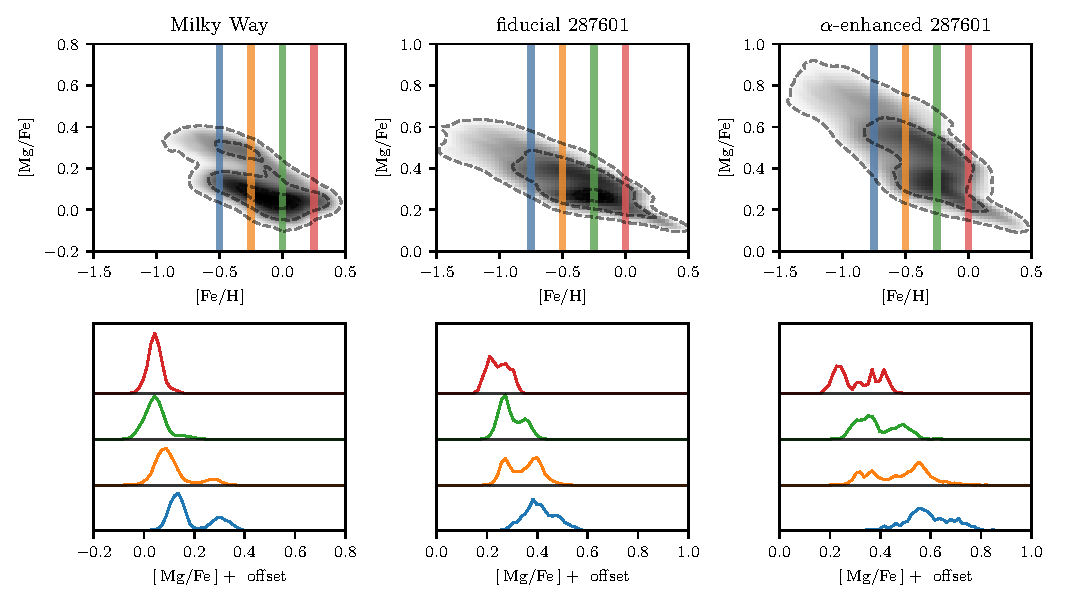
\includegraphics[width=\textwidth]{fig/app_287601.pdf}
  \caption{The same as Figure~\ref{fig:fig1}, but for a random subhalo from our catalog at $z=1.5$.}
  \label{fig:app15}
\end{figure*}

\begin{figure*}
  \centering
  \includegraphics[width=\textwidth]{fig/app_292983.pdf}
  \caption{The same as Figure~\ref{fig:fig1}, but for a random subhalo from our catalog at $z=1.5$.}
  \label{fig:app16}
\end{figure*}

\end{document}
